\documentclass{article}

\usepackage[hangul]{kotex}

\usepackage{multicol}

\usepackage{graphicx}

\usepackage{tcolorbox}
\tcbuselibrary{listings}

\usepackage{tikz}
\usepackage{makeshape}
\usepackage{flowchart}
\usetikzlibrary{arrows}

\newcommand{\code}[1]{
  \texttt{\large{#1}}
}

\title{기초공학설계 숫자 퍼즐 프로젝트}
\author{이주헌 (20191629)}
\date{2019년 6월 12일}

\begin{document}
\pagenumbering{gobble}
\maketitle
\newpage

\pagenumbering{arabic}

\section{개요}

이 프로그램은 실제 존재하는 슬라이딩 퍼즐(Sliding Puzzle)을 기반으로 만든 퍼즐 프로그램이다. 슬라이딩 퍼즐은 정사각형 모양의 보드와 작은 타일로 이루어져 있는데, 이 작은 타일을 원래 모양으로 되돌리는 것을 목적으로 하는 퍼즐이다.

\begin{figure}[ht!]
  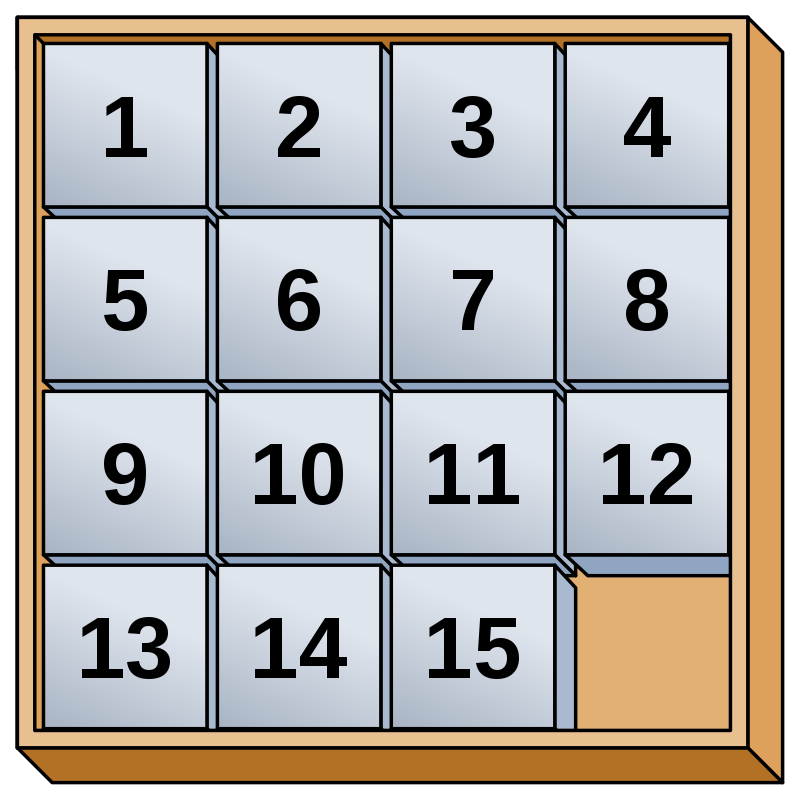
\includegraphics[width=\linewidth]{res/15-puzzle.png}
  \caption{슬라이딩 퍼즐의 일종인 15 퍼즐.}
  \label{fig:15-puzzle}
\end{figure}

슬라이딩 퍼즐은 직소 퍼즐과는 달리 타일을 보드로부터 떼어낼 수 없다. 실제 퍼즐은 플라스틱 조각을 맞붙여서 물리적으로 타일이 보드에서 떨어질 수 없게 만들어 둔 퍼즐이 많다. 따라서 타일을 보드에서 떼지 않고 움직이기 위해 한 공간은 비워져 있는데, 이 공간으로 타일을 밀어 넣음으로서 타일의 위치를 바꾼다.

보통 슬라이딩 퍼즐은 타일 조각 위에 숫자가 쓰여 있는 퍼즐이 대부분이지만, 경우에 따라 숫자 대신 그림이 그려져 있기도 하다. 이 때에는 그림을 원래 모양으로 복구하는 것이 목적이 된다.

하지만 이 프로그램에서는 숫자가 쓰여 있는 타일을 왼쪽 위부터 역순으로 정렬하는 것을 목표로 하는 슬라이딩 퍼즐을 구현한다.

\section{프로그램 구조}

숫자 퍼즐 프로그램에서 요구하는 사항은 다음과 같다.

\begin{enumerate}
\item 주어진 \code{puzzle\_student.c} 파일의 내용을 바꾸어 프로그램을 만들되, 이미 작성되어 있는 함수나 변수의 이름을 바꾸지 아니할 것.
\item 조작은 W, A, S, D 키로 하되, 빈칸을 채우는 방향으로 타일을 이동할 것.
\item 숫자가 왼쪽 위부터 내림차순으로 정렬되면 \code{Success!}를 출력하고 프로그램을 종료할 것.
\item 타일을 한 번씩 움직일 때마다 \code{Life}가 1씩 줄이고, 만약 \code{Life}가 0이 될 때까지 타일을 정렬하지 못하면 \code{Fail!}을 출력하고 프로그램을 종료할 것.
\item 주어진 테스트 케이스를 모두 통과하는 프로그램을 작성할 것.
\end{enumerate}

\subsection{프로그램 실행 흐름}

프로그램 실행부터 종료까지 흐름은 다음과 같다.

우선 시작 직후 게임판을 초기화한다. 게임판 초기화는 다시 두 단계로 나누어지는데, 첫 번째 단계는 보드의 상태를 저장하는 2차원 배열의 초기화이고, 두 번째 단계는 타일을 무작위로 움직여 보드를 섞는 작업이다.

초기화가 완료되면 게임 루프에 진입한다. 프로그램에 선언된 전역 변수 \code{game\_over}로부터 퍼즐이 풀렸는지 판단하고, 만약 풀리지 않았다면 다시 루프 안으로 진입한다. 만약 퍼즐이 풀렸다면 루프에서 빠져나와 \code{Success!}를 콘솔에 출력하고 프로그램을 종료한다.

게임 루프 안에서는 매 루프마다 사용자 입력을 받아 그에 알맞게 타일을 옮기는 작업을 한다. 이 때 \code{Life}를 1씩 줄여 나간다. 타일을 옮긴 뒤에는 게임판 배열로부터 게임 화면을 다시 그린다. 퍼즐이 풀렸는지 확인한 다음 알맞게 \code{game\_over} 전역 변수를 갱신한 뒤, \code{Life}가 더 남았는지 확인한다. 만약 \code{Life}가 0과 같거나 작다면 \code{Fail!}을 콘솔에 출력하고 프로그램을 종료한다. 만약 그렇지 않다면 루프의 처음으로 돌아가 퍼즐이 풀렸는지 검사한다.

\begin{figure}[h!]
  \centering
  \begin{tikzpicture}[>=latex', font={\sf \small}]
    
    \def\smbwd{2cm}
    
    \node (start-term) at (0, 0) [
      draw, terminal,
      minimum width = \smbwd,
      minimum height = 1cm
    ] {시작};
    
    \node (init) at (0, -1.5) [
      draw, process,
      minimum width = \smbwd,
      minimum height = 1cm
    ] {게임판 초기화하기};
    
    \node (is-gameover) at (0, -4) [
      draw, decision,
      minimum width = \smbwd*2,
      minimum height = 1cm
    ] {퍼즐이 풀렸는가?};
    
    \node (move-tile) at (0, -7) [
      draw, process,
      minimum width = \smbwd,
      minimum height = 1cm
    ] {사용자 입력을 받고 타일 옮기기};
    
    \coordinate (point1) at (-3.5, -8);
    
    \node (print-success) at (5, -8) [
      draw, process,
      minimum width = \smbwd,
      minimum height = 1cm
    ] {\code{Success!} 출력하기};
    
    \node (check-board) at (0, -8.5) [
      draw, process,
      minimum width = \smbwd,
      minimum height = 1cm
    ] {퍼즐이 풀렸는지 확인하기};
    
    \node (check-life) at (0, -10.5) [
      draw, decision,
      minimum width = \smbwd*2,
      minimum height = 1cm
    ] {\code{Life} $\leq$ 0};
    
    \node (print-fail) at (0, -13) [
      draw, process,
      minimum width = \smbwd,
      minimum height = 1cm
    ] {\code{Fail!} 출력하기};
    
    \coordinate (point3) at (0, -14);
    
    \node (end-term) at (0, -15) [
      draw, terminal,
      minimum width = \smbwd,
      minimum height = 1cm
    ] {끝};
    
    \draw[->] (start-term) -- (init);
    \draw[->] (init) -- (is-gameover);
    \draw[->] (is-gameover) -- node[left]{아니오} (move-tile);
    \draw[->] (is-gameover) -| node[above]{예} (print-success);
    \draw[->] (print-success) |- (point3);
    \draw[->] (move-tile) -- (check-board);
    \draw[->] (check-board) -- (check-life);
    \draw[->] (check-life) -- node[left]{예} (print-fail);
    \draw[-] (check-life) -| node[left]{아니오} (point1);
    \draw[->] (point1) |- (is-gameover);
    \draw[->] (print-fail) -- (end-term);
    
  \end{tikzpicture}
  \caption{프로그램의 전체 흐름도.}
  \label{fig:big-picture}
\end{figure}

\clearpage

\subsection{함수 목록과 기능}

이 프로그램에는 여러 함수가 사용되었으며, 각 함수의 기능은 다음과 같다.

\subsubsection{\code{main} 함수 (일부 구현 필요)}

\begin{tcblisting}{
    listing only,
    listing options = {
      basicstyle = \ttfamily,
      keywordstyle = \color{blue},
      language = c,
      columns = fullflexible,
      keepspaces = false
    },
    title = 함수 시그니처
  }int main(void);
\end{tcblisting}

프로그램의 시작점으로, 콘솔에서 명령어를 입력하면 가장 먼저 실행되는 함수이다. 퍼즐 보드를 선언하고 게임 루프를 실행하는 함수이며, 이 함수 안에서 다른 함수를 호출하여 게임을 구현한다. 이 함수에서 \code{Life}의 감소도 담당했는데, \code{move\_to} 함수의 성공 여부를 판단하여 만약 타일이 성공적으로 움직였다면 \code{Life}를 1씩 줄여 나간다.

게임 루프에 진입할 때 매번 \code{game\_over} 전역 변수를 확인하여 게임이 종료되었는지 확인하고, 만약 종료되었다면 \code{Success!}를 출력하고 프로그램을 정상 종료한다. 그렇지 않다면 사용자 입력을 받고 타일을 옮긴 뒤 퍼즐이 풀렸는지 확인하는 과정을 거친 뒤 \code{Life}가 0보다 작거나 같은지 확인한다. 만약 0보다 작거나 같다면 제한 명령 수 내에 퍼즐을 해결하지 못한 것이므로 \code{Fail!}을 출력하고 게임을 종료한다. 그렇지 않다면 아직 제한 명령 개수가 남은 것이므로 다시 게임 루프의 처음으로 돌아가서 \code{game\_over} 전역 변수를 확인하는 과정을 거친다.

\subsubsection{\code{init} 함수 (구현 불필요)}

\begin{tcblisting}{
    listing only,
    listing options = {
      basicstyle = \ttfamily,
      keywordstyle = \color{blue},
      language = c,
      columns = fullflexible
    },
    title = 함수 시그니처
  }void init(int puzzle[][size]);
\end{tcblisting}

\code{main} 함수에서 선언한 퍼즐 보드를 인자로 받아 보드를 초기화하고 \code{game\_over} 전역 변수를 초기화하는 함수이다. 초기화 된 후의 보드는 전부 맞춰져 있는 상태이며, 빈칸은 0으로 설정되어 있다.

\subsubsection{\code{printPuzzle} 함수 (구현 불필요)}

\begin{tcblisting}{
    listing only,
    listing options = {
      basicstyle = \ttfamily,
      keywordstyle = \color{blue},
      language = c,
      columns = fullflexible
    },
    title = 함수 시그니처
  }void printPuzzle(int puzzle[][size]);
\end{tcblisting}

퍼즐 보드 2차원 배열을 인자로 받아 보드를 실제로 화면에 그리는 역할을 하는 함수이다. 먼저 화면을 지우고 \code{size} 매크로 상수를 바탕으로 반복해서 + 문자와 - 문자를 이용해 퍼즐 보드를 그린다.

\subsubsection{\code{checkPuzzle} 함수}

\begin{tcblisting}{
    listing only,
    listing options = {
      basicstyle = \ttfamily,
      keywordstyle = \color{blue},
      language = c,
      columns = fullflexible
    },
    title = 함수 시그니처
  }void checkPuzzle(int puzzle[][size]);
\end{tcblisting}

퍼즐 보드 2차원 배열을 인자로 받아 퍼즐이 풀렸는지 확인하는 함수이다. 왼쪽 위 타일부터 오른쪽으로 순회하면서 숫자가 1씩 작아지는지 확인하는 방식으로 퍼즐의 해결 여부를 검사한다. 반복 도중 만약 예상과 다른 숫자가 감지될 경우 \code{game\_over} 전역 변수를 0으로 설정하고 즉시 반환한다. 도중에 반환되지 않고 끝까지 반복문을 수행한 경우 퍼즐이 풀린 것으로 보고 \code{game\_over} 전역 변수를 1으로 설정하고 반환한다.

\subsubsection{\code{find\_0\_loc} 함수}

\begin{tcblisting}{
    listing only,
    listing options = {
      basicstyle = \ttfamily,
      keywordstyle = \color{blue},
      language = c,
      columns = fullflexible
    },
    title = 함수 시그니처
  }int find_0_loc(int puzzle[][size]);
\end{tcblisting}

퍼즐 보드 2차원 배열을 인자로 받아 퍼즐 보드에서 0의 위치, 즉 빈칸의 위치를 구하는 함수이다. 퍼즐 보드의 모든 타일을 순차적으로 확인하면서 0을 발견하면 그 위치를 반환하는 함수이다. 그러나 C에서는 여러 값을 한 번에 반환할 수 없고, 제약 조건 상 주어진 함수 시그니처도 바꿀 수 없으므로 0의 위치를 하나의 정수 값으로 표현했다. \code{size}는 컴파일 타임 상수이므로 실행 도중 값이 바뀌지 않을 것이 명확하고, 이 상수에 따라 게임 보드의 크기가 결정되므로 다음 식을 이용해서 빈칸의 위치를 나타냈다.

\begin{equation}
  \label{eq:0-loc-equation}
  location = row * \texttt{size} + column
\end{equation}

\subsubsection{\code{getch} 함수 (구현 불필요)}

\begin{tcblisting}{
    listing only,
    listing options = {
      basicstyle = \ttfamily,
      keywordstyle = \color{blue},
      language = c,
      columns = fullflexible
    },
    title = 함수 시그니처
  }int getch(void);
\end{tcblisting}

터미널 제어 함수를 사용해서 터미널에 글자를 출력하지 않고 입력한 글자를 받아오는 함수이다. 만약 오류가 발생했을 경우 -1을 반환하므로 \code{char} 타입이 아닌 \code{int} 타입을 반환하도록 만들어져 있다. 따라서 반환값이 0보다 크거나 같다면 \code{char} 타입으로 캐스팅해도 무방하다.

\subsubsection{\code{move\_to} 함수}

\begin{tcblisting}{
    listing only,
    listing options = {
      basicstyle = \ttfamily,
      keywordstyle = \color{blue},
      language = c,
      columns = fullflexible
    },
    title = 함수 시그니처
  }int move_to(int puzzle[][size], int loc, int command);
\end{tcblisting}

퍼즐 보드 2차원 배열과 빈칸의 위치, 그리고 플레이어의 명령을 인자로 받아 타일을 옮기는 함수이다. 빈칸의 위치는 \code{find\_0\_loc} 함수의 반환값을 사용하므로, 위에서 정의한 식 \ref{eq:0-loc-equation}으로부터 빈칸의 행, 열 위치를 알 수 있다. 먼저 플레이어의 명령에 따라 5가지 경우로 분기하는데, 명령이 \code{Q}일 경우 퍼즐을 포기했다는 의미이므로 타일을 더 이상 옮기지 않고 오류 코드 \code{0xF}와 함께 프로그램을 종료한다.\footnote{이 부분은 사양에 존재하지 않는 기능이지만 디버깅 시에 매번 SIGINT 신호를 보내는 것이 불편해서 추가한 기능이다.} 다른 유효한 이동 명령은 먼저 타일을 옮겼을 때 빈칸이 유효한 위치에 있을지 검사한 뒤 실제로 타일의 위치를 변경한다. 만약 유효하지 않은 명령일 경우 아무것도 하지 않고 -1을 반환한다.

\subsubsection{\code{shuffle} 함수 (구현 불필요)}

\begin{tcblisting}{
    listing only,
    listing options = {
      basicstyle = \ttfamily,
      keywordstyle = \color{blue},
      language = c,
      columns = fullflexible
    },
    title = 함수 시그니처
  }void shuffle(int puzzle[][size]);
\end{tcblisting}

퍼즐 보드 2차원 배열을 인자로 받아 보드를 무작위로 섞는 함수이다. \code{rand} 함수를 이용해서 난수를 생성하고 이 난수로부터 임의로 사용자 입력을 생성한 뒤 \code{find\_0\_loc} 함수와 \code{move\_to} 함수를 이용해서 타일을 무작위로 옮긴다. 따라서 이 함수는 \code{find\_0\_loc} 함수와 \code{move\_to} 함수가 올바르게 구현되어 있는 것을 전제로 한다. 이 절차를 여러 번 반복하는데, 100회 반복을 기본으로 하고, 필요에 따라 값을 변경할 수 있다.

\subsubsection{\code{GetCommand} 함수 (구현 불필요)}

\begin{tcblisting}{
    listing only,
    listing options = {
      basicstyle = \ttfamily,
      keywordstyle = \color{blue},
      language = c,
      columns = fullflexible
    },
    title = 함수 시그니처
  }int GetCommand();
\end{tcblisting}

\code{getch} 함수로부터 입력한 키 값을 가져오고 그 값을 명령 플래그로 바꿔주는 함수이다. 0은 위, 1은 왼쪽, 2는 아래, 3은 오른쪽 방향 명령을 의미한다. \code{Q}를 입력한 경우 게임 포기로 간주하고 9를 반환한다.\footnote{원래 없는 코드 조각이지만 \texttt{move\_to} 함수에서의 사용을 위해 추가했다.} 만약 유효한 키가 아닌 다른 키가 입력되면 -1을 반환한다.

\end{document}
